\documentclass[12pt, titlepage]{article}

\usepackage{fullpage}
\usepackage[round]{natbib}
\usepackage{multirow}
\usepackage{booktabs}
\usepackage{tabularx}
\usepackage{graphicx}
\usepackage{float}
\usepackage{hyperref}
\hypersetup{
    colorlinks,
    citecolor=black,
    filecolor=black,
    linkcolor=red,
    urlcolor=blue
}
\usepackage[round]{natbib}

\newcounter{acnum}
\newcommand{\actheacnum}{AC\theacnum}
\newcommand{\acref}[1]{AC\ref{#1}}

\newcounter{ucnum}
\newcommand{\uctheucnum}{UC\theucnum}
\newcommand{\uref}[1]{UC\ref{#1}}

\newcounter{mnum}
\newcommand{\mthemnum}{M\themnum}
\newcommand{\mref}[1]{M\ref{#1}}

\title{SE 3XA3: Design Document\\Mari0}

\author{Team 9, Ninetendo
		\\ David Hobson hobsondd
		\\ Jose Miguel Ballesteros ballesjm
		\\ Jeff Pineda pinedaj
}

\date{\today}

%% Comments

\usepackage{color}

\newif\ifcomments\commentstrue

\ifcomments
\newcommand{\authornote}[3]{\textcolor{#1}{[#3 ---#2]}}
\newcommand{\todo}[1]{\textcolor{red}{[TODO: #1]}}
\else
\newcommand{\authornote}[3]{}
\newcommand{\todo}[1]{}
\fi

\newcommand{\wss}[1]{\authornote{blue}{SS}{#1}}
\newcommand{\ds}[1]{\authornote{red}{DS}{#1}}
\newcommand{\mj}[1]{\authornote{red}{MSN}{#1}}
\newcommand{\cm}[1]{\authornote{red}{CM}{#1}}
\newcommand{\mh}[1]{\authornote{red}{MH}{#1}}

% team members should be added for each team, like the following
% all comments left by the TAs or the instructor should be addressed
% by a corresponding comment from the Team

\newcommand{\tm}[1]{\authornote{magenta}{Team}{#1}}


\begin{document}

\maketitle

\pagenumbering{roman}
\tableofcontents
\listoftables
\listoffigures

\begin{table}[bp]
\caption{\bf Revision History}
\begin{tabularx}{\textwidth}{p{3cm}p{2cm}X}
\toprule {\bf Date} & {\bf Version} & {\bf Notes}\\
\midrule
2016-11-13 & 1.0 & Creation of rev0\\
\bottomrule
\end{tabularx}
\end{table}

\newpage

\pagenumbering{arabic}

\section{Introduction}

Decomposing a system into modules is a commonly accepted approach to developing
software.  A module is a work assignment for a programmer or programming
team~\citep{ParnasEtAl1984}.  We advocate a decomposition
based on the principle of information hiding~\citep{Parnas1972a}.  This
principle supports design for change, because the ``secrets'' that each module
hides represent likely future changes.  Design for change is valuable in SC,
where modifications are frequent, especially during initial development as the
solution space is explored.  

Our design follows the rules layed \textcolor{red}{should this be laid? - CM} \\ out by \citet{ParnasEtAl1984}, as follows:
\begin{itemize}
\item System details that are likely to change independently should be the
  secrets of separate modules.
\item Each data structure is used in only one module.
\item Any other program that requires information stored in a module's data
  structures must obtain it by calling access programs belonging to that module.
\end{itemize}

After completing the first stage of the design, the Software Requirements
Specification (SRS), the Module Guide (MG) is developed~\citep{ParnasEtAl1984}. The MG
specifies the modular structure of the system and is intended to allow both
designers and maintainers to easily identify the parts of the software.  The
potential readers of this document are as follows:

\begin{itemize}
\item New project members: This document can be a guide for a new project member
  to easily understand the overall structure and quickly find the
  relevant modules they are searching for.
\item Maintainers: The hierarchical structure of the module guide improves the
  maintainers' understanding when they need to make changes to the system. It is
  important for a maintainer to update the relevant sections of the document
  after changes have been made.
\item Designers: Once the module guide has been written, it can be used to
  check for consistency, feasibility and flexibility. Designers can verify the
  system in various ways, such as consistency among modules, feasibility of the
  decomposition, and flexibility of the design.
\end{itemize}

The rest of the document is organized as follows. Section
\ref{SecChange} lists the anticipated and unlikely changes of the software
requirements. Section \ref{SecMH} summarizes the module decomposition that
was constructed according to the likely changes. Section \ref{SecConnection}
specifies the connections between the software requirements and the
modules. Section \ref{SecMD} gives a detailed description of the
modules. Section \ref{SecTM} includes two traceability matrices. One checks
the completeness of the design against the requirements provided in the SRS. The
other shows the relation between anticipated changes and the modules. Section
\ref{SecUse} describes the use relation between modules.

\section{Anticipated and Unlikely Changes} \label{SecChange}
This section shows some of the upcoming changes to Mari0 listed into two categories. 
Anticipated changes are listed in Section \ref{SecAchange}, and
unlikely changes are listed in Section \ref{SecUchange}.

\subsection{Anticipated Changes} \label{SecAchange}

Some of the changes below are what we believe will be implemented as development continues. Due to the modularization of our software, many of the changes that will happen will be simple and allow the system to function properly.

\begin{description}
\item[\refstepcounter{acnum} \actheacnum \label{acEnvironments}:] Level Environments. All of the levels that will be created will be unique and making sure that game objects interact properly is crucial.
\item[\refstepcounter{acnum} \actheacnum \label{acEnemiest}:] Types of Enemies. Adding new enemies in the game is expected and is considered in the design.
\item [\refstepcounter{acnum} \actheacnum \label{acOperatingSys}:] Operating System. All operating systems will be supported and allowing the software to be dynamic and run on these systems is important.
\item [\refstepcounter{acnum} \actheacnum \label{acMusic}:] Music and Sound Effects. These will be changed based off of different environmental factors of the game.
\end{description}

\subsection{Unlikely Changes} \label{SecUchange}

The changes listed below are changes that will not be considered as important for the final product and demonstration.

\begin{description}
\item[\refstepcounter{ucnum} \uctheucnum \label{ucPlatform}:] Platform. For this game, the only platform that it will run on will be a personal computer, although operating systems may change, this game will not run on mobile or game console devices.
\item[\refstepcounter{ucnum} \uctheucnum \label{ucSprites}:] Sprites/Models. Although in the original game there?s customization available for sprites, this will not be considered in our design.
\item[\refstepcounter{ucnum} \uctheucnum \label{ucMechanics}:] Game Mechanics. The basic idea of the game will stay as a platformer with the player walking to the right and interacting with different obstacles.
\end{description}

\section{Module Hierarchy} \label{SecMH}

This section provides an overview of the module design. Modules are summarized
in a hierarchy decomposed by secrets in Table \ref{TblMH}. The modules listed
below, which are leaves in the hierarchy tree, are the modules that will
actually be implemented.

\begin{description}
\item [\refstepcounter{mnum} \mthemnum \label{mHH}:] Hardware-Hiding Module
\item  [\refstepcounter{mnum} \mthemnum \label{mMI}:] Mouse Input Module
\item  [\refstepcounter{mnum} \mthemnum \label{mKI}:] Keyboard Input Module
\item  [\refstepcounter{mnum} \mthemnum \label{mInput}:] Input Format Module
\item  [\refstepcounter{mnum} \mthemnum \label{mPP}:] Portal Phyiscs \textcolor{red}{Typo - CM} \\ Module
\item  [\refstepcounter{mnum} \mthemnum \label{mPG}:] Portal Gun Module
\item  [\refstepcounter{mnum} \mthemnum \label{mGO}:] Game Object Module
\item  [\refstepcounter{mnum} \mthemnum \label{mPO}:] Player Object Module
\item  [\refstepcounter{mnum} \mthemnum \label{mSM}:] Sprite/Model Module
\item  [\refstepcounter{mnum} \mthemnum \label{mInterface}:] Interface Module
\item  [\refstepcounter{mnum} \mthemnum \label{mCD}:] Collision Detection Module
\end{description}

\begin{table}[h!]
\centering
\begin{tabular}{p{0.3\textwidth} p{0.6\textwidth}}
\toprule
\textbf{Level 1} & \textbf{Level 2}\\
\midrule

{Hardware-Hiding Module} & ~ \\
\midrule

\multirow{7}{0.3\textwidth}{Behaviour-Hiding Module}
& Collision Detection Module\\
& Event Input Module\\
& Interface Module\\
& Sprite/Model Module\\
\midrule

\multirow{3}{0.3\textwidth}{Software Decision Module}
& Portal Physics Module \textcolor{red}{If this pertains to your SRS, it does not belong here. Move up one cell. - CM} \\\\
& Game Object Module\\
& Player Object Module\\
\bottomrule

\end{tabular}
\caption{Module Hierarchy}
\label{TblMH}
\end{table}

\section{Connection Between Requirements and Design} \label{SecConnection}

The design of the system is intended to satisfy the requirements developed in
the SRS. In this stage, the system is decomposed into modules. The connection
between requirements and modules is listed in Table \ref{TblRT}.

\section{Module Decomposition} \label{SecMD}

Modules are decomposed according to the principle of ``information hiding''
proposed by \citet{ParnasEtAl1984}. The \emph{Secrets} field in a module
decomposition is a brief statement of the design decision hidden by the
module. The \emph{Services} field specifies \emph{what} the module will do
without documenting \emph{how} to do it. For each module, a suggestion for the
implementing software is given under the \emph{Implemented By} title. If the
entry is \emph{OS}, this means that the module is provided by the operating
system or by standard programming language libraries.  Also indicate if the
module will be implemented specifically for the software.

Only the leaf modules in the
hierarchy have to be implemented. If a dash (\emph{--}) is shown, this means
that the module is not a leaf and will not have to be implemented. Whether or
not this module is implemented depends on the programming language
selected.

\subsection{Hardware Hiding Modules (\mref{mHH})}

\begin{description}
\item[Secrets:]The data structure and algorithm used to implement the virtual
  hardware.
\item[Services:]Serves as a virtual hardware used by the rest of the
  system. This module provides the interface between the hardware and the
  software. So, the system can use it to display outputs or to accept inputs.
\item[Implemented By:] OS
\end{description}

\subsubsection{Mouse Inputs (\mref{mMI})}

\begin{description}
\item[Secrets:] How mouse input is used in relation to the computer \textcolor{red}{These should be nouns! - CM} \\
\item[Services:] Player mouse inputs are displayed on-screen 
\item[Implemented By:] OS
\end{description}

\subsubsection{Keyboard Inputs (\mref{mKI})}

\begin{description}
\item[Secrets:] How keyboard input is used in relation to the computer
\item[Services:] Player keyboard inputs are displayed on-screen 
\item[Implemented By:] OS
\end{description}



\subsection{Behaviour-Hiding Module}

\begin{description}
\item[Secrets:]The contents of the required behaviours.
\item[Services:]Includes programs that provide externally visible behaviour of
  the system as specified in the software requirements specification (SRS)
  documents. This module serves as a communication layer between the
  hardware-hiding module and the software decision module. The programs in this
  module will need to change if there are changes in the SRS.
\item[Implemented By:] --
\end{description}

\subsubsection{Input Format Module (\mref{mInput})}

\begin{description}
\item[Secrets:]The format and structure of the input data.
\item[Services:]Converts the input data into the data structure used by the
  input parameters module.
\item[Implemented By:] Mari0
\end{description}

\subsubsection{Portal Physics Module (\mref{mPP})}
\begin{description}
\item[Secrets:] How teleportation between two portals works and the game entities that can enter a portal
\item[Services:] Teleports game entities that can be teleported between two portals
\item[Implemented By:] Mari0
\end{description}

\subsubsection{Portal Gun Module (\mref{mPG})}
\begin{description}
\item[Secrets:] The coordinates of both the blue and the orange portal, and the coordinates of the surface the player is aiming at \textcolor{red}{If this requires to things, the module should be split. Or reword to just have one thing - CM} \\
\item[Services:] Allows the player to aim and place either a blue portal or an orange portal on a surface
\item[Implemented By:] Mari0
\end{description}

\subsubsection{Game Object Module (\mref{mGO})}
\begin{description}
\item[Secrets: ]The size and coordinates of the game object
\item[Services:]Allows size and coordinates to be changed and be interacted with by the player
\item[Implemented By:] Mari0
\end{description}

\subsubsection{Player Object Module (\mref{mPO})}
\begin{description}
\item[Secrets:]Size, coordinates of player object, player status (alive or dead), and player attributes such as speed, jump force, and gravity.
\item[Services:]Allows size and coordinates to be changed and be interacted with by the player and keeps track of player status
\item[Implemented By:] Mari0
\end{description}

\subsection{Software Decision Module}

\begin{description}
\item[Secrets:] The design decision based on mathematical theorems, physical
  facts, or programming considerations. The secrets of this module are
  \emph{not} described in the SRS.
\item[Services:] Includes data structure and algorithms used in the system that
  do not provide direct interaction with the user. 
  % Changes in these modules are more likely to be motivated by a desire to
  % improve performance than by externally imposed changes.
\item[Implemented By:] --
\end{description}

\subsubsection{Sprite/Model Module (\mref{mSM})}
\begin{description}
\item[Secrets:]How sprites and models are displayed in game
\item[Services:]Displays sprites and models in game
\item[Implemented By:] Mari0
\end{description}

\subsubsection{Interface Module (\mref{mInterface})}
\begin{description}
\item[Secrets:]Information about the game, such as time left, points scored, and current level
\item[Services:]Keeps track of and displays game time, score, and current level
\item[Implemented By:] Mari0
\end{description}

\subsubsection{Collision Detectionl Module (\mref{mCD}) \textcolor{red}{Typo - CM} \\}
\begin{description}
\item[Secrets:]How collision is calculated \textcolor{red}{Noun! Just say, Collision Mechanics - CM} \\
\item[Services:]Determines whether two entities in the game are touching or will eventually touch one another
\item[Implemented By:] Mari0
\end{description}

\section{Traceability Matrix} \label{SecTM}

This section shows two traceability matrices: between the modules and the
requirements and between the modules and the anticipated changes.

% the table should use mref, the requirements should be named, use something
% like fref
\begin{table}[H]
\centering
\begin{tabular}{p{0.2\textwidth} p{0.6\textwidth}}
\toprule
\textbf{Req.} & \textbf{Modules}\\
\midrule
R1 & \mref{mHH}, \mref{mInput}, \mref{mParams}, \mref{mControl}\\
R2 & \mref{mInput}, \mref{mParams}\\
R3 & \mref{mVerify} \textcolor{red}{These aren't labelled anywhere... Did you not remove these? - CM} \\\\
R4 & \mref{mOutput}, \mref{mControl}\\
R5 & \mref{mOutput}, \mref{mODEs}, \mref{mControl}, \mref{mSeqDS}, \mref{mSolver}, \mref{mPlot}\\
R6 & \mref{mOutput}, \mref{mODEs}, \mref{mControl}, \mref{mSeqDS}, \mref{mSolver}, \mref{mPlot}\\
R7 & \mref{mOutput}, \mref{mEnergy}, \mref{mControl}, \mref{mSeqDS}, \mref{mPlot}\\
R8 & \mref{mOutput}, \mref{mEnergy}, \mref{mControl}, \mref{mSeqDS}, \mref{mPlot}\\
R9 & \mref{mVerifyOut}\\
R10 & \mref{mOutput}, \mref{mODEs}, \mref{mControl}\\
R11 & \mref{mOutput}, \mref{mODEs}, \mref{mEnergy}, \mref{mControl}\\
\bottomrule
\end{tabular}
\caption{Trace Between Requirements and Modules}
\label{TblRT}
\end{table}

\begin{table}[H]
\centering
\begin{tabular}{p{0.2\textwidth} p{0.6\textwidth}}
\toprule
\textbf{AC} & \textbf{Modules}\\
\midrule
\acref{acHardware} & \mref{mHH}\\
\acref{acInput} & \mref{mInput}\\
\acref{acParams} & \mref{mParams}\\
\acref{acVerify} & \mref{mVerify}\\
\acref{acOutput} & \mref{mOutput}\\
\acref{acVerifyOut} & \mref{mVerifyOut}\\
\acref{acODEs} & \mref{mODEs}\\
\acref{acEnergy} & \mref{mEnergy}\\
\acref{acControl} & \mref{mControl}\\
\acref{acSeqDS} & \mref{mSeqDS}\\
\acref{acSolver} & \mref{mSolver}\\
\acref{acPlot} & \mref{mPlot}\\
\bottomrule
\end{tabular}
\caption{Trace Between Anticipated Changes and Modules}
\label{TblACT}
\end{table}

\section{Use Hierarchy Between Modules} \label{SecUse}

In this section, the uses hierarchy between modules is
provided. \citet{Parnas1978} said of two programs A and B that A {\em uses} B if
correct execution of B may be necessary for A to complete the task described in
its specification. That is, A {\em uses} B if there exist situations in which
the correct functioning of A depends upon the availability of a correct
implementation of B.  Figure \ref{FigUH} illustrates the use relation between
the modules. It can be seen that the graph is a directed acyclic graph
(DAG). Each level of the hierarchy offers a testable and usable subset of the
system, and modules in the higher level of the hierarchy are essentially simpler
because they use modules from the lower levels.

\begin{figure}[H]
\centering
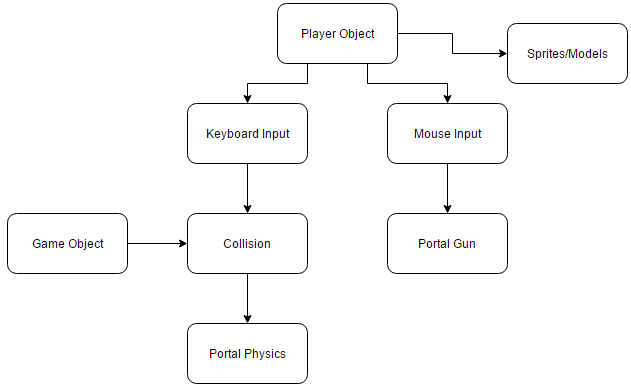
\includegraphics[width=0.7\textwidth]{UsesHierarchy.png}
\caption{Use hierarchy among modules}
\label{FigUH}
\end{figure}

%\section*{References}

\bibliographystyle {plainnat}
\bibliography {MG}

\end{document}